\chapter{Recorreguts en grafs}

Aquest capítol tracta dos algorismes fonamentals de grafs: la cerca
en profunditat i la cerca en amplada. Ambdós algorismes reben un
node inicial del graf i visiten tots els nodes als quals es pot
accedir des del node inicial. La diferència entre els algorismes és
l'ordre en què visiten els nodes.

\section{Cerca en profunditat}

\index{cerca en profunditat}

\key{Cerca en profunditat} (\emph{depth-first search}, DFS) és una
tècnica senzilla per a recórrer grafs. L'algorisme comença en un node
inicial, i continua per tots els altres nodes als quals es pot accedir
des del node inicial fent servir les arestes del graf.

La cerca en profunditat sempre recorre un únic camí del graf mentre
trobi nodes nous per explorar. Després d'això, torna als nodes
anteriors i comença a explorar altres parts del graf. L'algoritme té
control dels nodes que ja han estat visitats, de manera que processa
cada node només una vegada.

\subsubsection*{Exemple}

Posem com a exemple la cerca en profunditat del graf següent:
\begin{center}
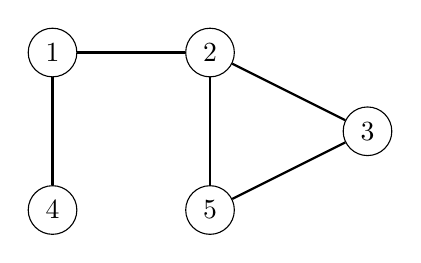
\begin{tikzpicture}
\node[draw, circle] (1) at (1,5) {$1$};
\node[draw, circle] (2) at (3,5) {$2$};
\node[draw, circle] (3) at (5,4) {$3$};
\node[draw, circle] (4) at (1,3) {$4$};
\node[draw, circle] (5) at (3,3) {$5$};

\path[draw,thick,-] (1) -- (2);
\path[draw,thick,-] (2) -- (3);
\path[draw,thick,-] (1) -- (4);
\path[draw,thick,-] (3) -- (5);
\path[draw,thick,-] (2) -- (5);
\end{tikzpicture}
\end{center}
Podem començar la cerca en qualsevol node del graf, per exemple, el
node 1.

La cerca passa primer pel node 2:
\begin{center}
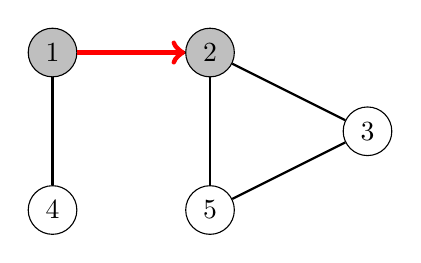
\begin{tikzpicture}
\node[draw, circle,fill=lightgray] (1) at (1,5) {$1$};
\node[draw, circle,fill=lightgray] (2) at (3,5) {$2$};
\node[draw, circle] (3) at (5,4) {$3$};
\node[draw, circle] (4) at (1,3) {$4$};
\node[draw, circle] (5) at (3,3) {$5$};

\path[draw,thick,-] (1) -- (2);
\path[draw,thick,-] (2) -- (3);
\path[draw,thick,-] (1) -- (4);
\path[draw,thick,-] (3) -- (5);
\path[draw,thick,-] (2) -- (5);

\path[draw=red,thick,->,line width=2pt] (1) -- (2);
\end{tikzpicture}
\end{center}
Després d'això, visita els nodes 3 i 5:
\begin{center}
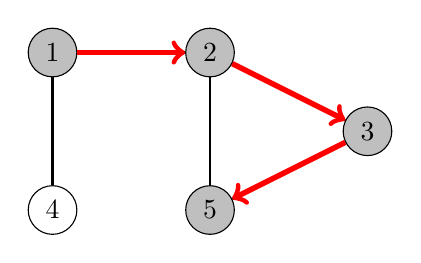
\begin{tikzpicture}
\node[draw, circle,fill=lightgray] (1) at (1,5) {$1$};
\node[draw, circle,fill=lightgray] (2) at (3,5) {$2$};
\node[draw, circle,fill=lightgray] (3) at (5,4) {$3$};
\node[draw, circle] (4) at (1,3) {$4$};
\node[draw, circle,fill=lightgray] (5) at (3,3) {$5$};

\path[draw,thick,-] (1) -- (2);
\path[draw,thick,-] (2) -- (3);
\path[draw,thick,-] (1) -- (4);
\path[draw,thick,-] (3) -- (5);
\path[draw,thick,-] (2) -- (5);

\path[draw=red,thick,->,line width=2pt] (1) -- (2);
\path[draw=red,thick,->,line width=2pt] (2) -- (3);
\path[draw=red,thick,->,line width=2pt] (3) -- (5);
\end{tikzpicture}
\end{center}
Els veïns del node 5 són el 2 i el 3, però la cerca ja ha visitat
ambdós, de manera que tornem als nodes anteriors. També hem vist els
veïns dels nodes 3 i 2, per la qual cosa el següent moviment és del
node 1 al node 4:
\begin{center}
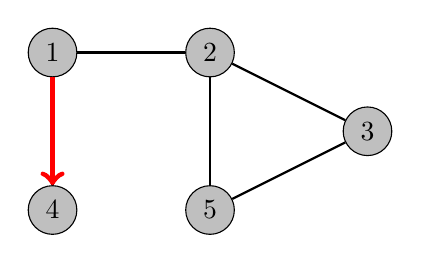
\begin{tikzpicture}
\node[draw, circle,fill=lightgray] (1) at (1,5) {$1$};
\node[draw, circle,fill=lightgray] (2) at (3,5) {$2$};
\node[draw, circle,fill=lightgray] (3) at (5,4) {$3$};
\node[draw, circle,fill=lightgray] (4) at (1,3) {$4$};
\node[draw, circle,fill=lightgray] (5) at (3,3) {$5$};

\path[draw,thick,-] (1) -- (2);
\path[draw,thick,-] (2) -- (3);
\path[draw,thick,-] (1) -- (4);
\path[draw,thick,-] (3) -- (5);
\path[draw,thick,-] (2) -- (5);

\path[draw=red,thick,->,line width=2pt] (1) -- (4);
\end{tikzpicture}
\end{center}
Després d'això, la cerca finalitza perquè ha visitat tots els nodes.

La complexitat temporal de la cerca en profunditat és $O(n+m)$ on $n$
és el nombre de nodes i $m$ és el nombre d'arestes, perquè l'algorisme
processa cada node i aresta una sola vegada.

\subsubsection*{Implementació}

La cerca en profunditat es pot implementar còmodament mitjançant
recursivitat. La següent funció \texttt{dfs} comença una cerca en
profunditat en un node determinat. La funció suposa que el graf
s'emmagatzema com a llistes d'adjacència en un vector
\begin{lstlisting}
vector<int> adj[N];
\end{lstlisting}
i també manté un vector
\begin{lstlisting}
bool visited[N];
\end{lstlisting}
per conèixer els nodes visitats. Inicialment, cada valor del vector és
\texttt{false}, i quan la cerca arriba al node $s$, el valor de
\texttt{visited}[$s$] es converteix en \texttt{true}. La funció es pot
implementar de la següent manera:
\begin{lstlisting}
void dfs(int s) {
    if (visited[s]) return;
    visited[s] = true;
    // process node s
    for (auto u: adj[s]) {
        dfs(u);
    }
}
\end{lstlisting}


\section{Cerca en amplada}

\index{cerca en amplada}

La \key{cerca en amplada} (\emph{breadth-first search}, BFS) visita
els nodes en ordre creixent a la seva distància des del node
inicial. Així, podem calcular la distància des del node inicial fins a
la resta de nodes mitjançant la cerca en amplada. Tanmateix, la cerca
en amplada és més difícil d'implementar que la cerca en profunditat.

La cerca en amplada passa per tots els nodes d'un nivell abans de
considerar els nodes del nivell següent. Primer, la cerca explora tots
els nodes a distància 1 del node inicial, després els nodes a
distància 2, i així successivament. Aquest procés continua fins que
s'han visitat tots els nodes.

\subsubsection*{Exemple}

Considerem com la cerca en amplada processa el graf següent:


\begin{center}
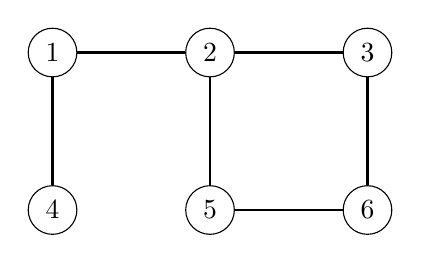
\begin{tikzpicture}
\node[draw, circle] (1) at (1,5) {$1$};
\node[draw, circle] (2) at (3,5) {$2$};
\node[draw, circle] (3) at (5,5) {$3$};
\node[draw, circle] (4) at (1,3) {$4$};
\node[draw, circle] (5) at (3,3) {$5$};
\node[draw, circle] (6) at (5,3) {$6$};

\path[draw,thick,-] (1) -- (2);
\path[draw,thick,-] (2) -- (3);
\path[draw,thick,-] (1) -- (4);
\path[draw,thick,-] (3) -- (6);
\path[draw,thick,-] (2) -- (5);
\path[draw,thick,-] (5) -- (6);
\end{tikzpicture}
\end{center}
Suposem que la cerca comença al node 1. En primer lloc, processem tots
els nodes als quals es pot arribar des del node 1 mitjançant una única
aresta:
\begin{center}
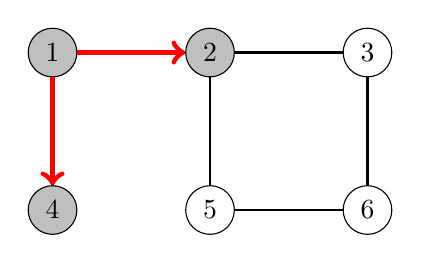
\begin{tikzpicture}
\node[draw, circle,fill=lightgray] (1) at (1,5) {$1$};
\node[draw, circle,fill=lightgray] (2) at (3,5) {$2$};
\node[draw, circle] (3) at (5,5) {$3$};
\node[draw, circle,fill=lightgray] (4) at (1,3) {$4$};
\node[draw, circle] (5) at (3,3) {$5$};
\node[draw, circle] (6) at (5,3) {$6$};

\path[draw,thick,-] (1) -- (2);
\path[draw,thick,-] (2) -- (3);
\path[draw,thick,-] (1) -- (4);
\path[draw,thick,-] (3) -- (6);
\path[draw,thick,-] (2) -- (5);
\path[draw,thick,-] (5) -- (6);

\path[draw,thick,-] (1) -- (2);
\path[draw,thick,-] (2) -- (3);
\path[draw,thick,-] (1) -- (4);
\path[draw,thick,-] (2) -- (5);

\path[draw=red,thick,->,line width=2pt] (1) -- (2);
\path[draw=red,thick,->,line width=2pt] (1) -- (4);
\end{tikzpicture}
\end{center}
Després d'això, passem als nodes 3 i 5:
\begin{center}
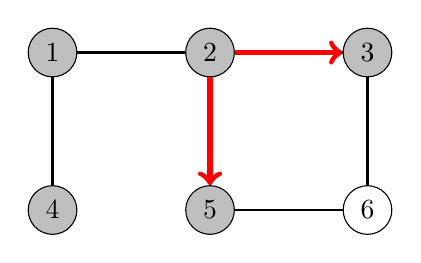
\begin{tikzpicture}
\node[draw, circle,fill=lightgray] (1) at (1,5) {$1$};
\node[draw, circle,fill=lightgray] (2) at (3,5) {$2$};
\node[draw, circle,fill=lightgray] (3) at (5,5) {$3$};
\node[draw, circle,fill=lightgray] (4) at (1,3) {$4$};
\node[draw, circle,fill=lightgray] (5) at (3,3) {$5$};
\node[draw, circle] (6) at (5,3) {$6$};

\path[draw,thick,-] (1) -- (2);
\path[draw,thick,-] (2) -- (3);
\path[draw,thick,-] (1) -- (4);
\path[draw,thick,-] (3) -- (6);
\path[draw,thick,-] (2) -- (5);
\path[draw,thick,-] (5) -- (6);

\path[draw,thick,-] (1) -- (2);
\path[draw,thick,-] (2) -- (3);
\path[draw,thick,-] (1) -- (4);
\path[draw,thick,-] (2) -- (5);

\path[draw=red,thick,->,line width=2pt] (2) -- (3);
\path[draw=red,thick,->,line width=2pt] (2) -- (5);
\end{tikzpicture}
\end{center}
Finalment, visitem el node 6:
\begin{center}
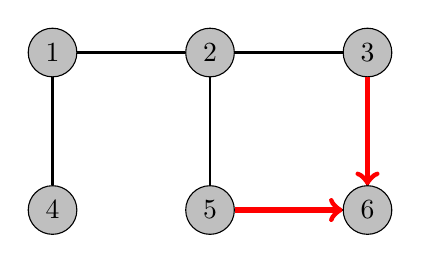
\begin{tikzpicture}
\node[draw, circle,fill=lightgray] (1) at (1,5) {$1$};
\node[draw, circle,fill=lightgray] (2) at (3,5) {$2$};
\node[draw, circle,fill=lightgray] (3) at (5,5) {$3$};
\node[draw, circle,fill=lightgray] (4) at (1,3) {$4$};
\node[draw, circle,fill=lightgray] (5) at (3,3) {$5$};
\node[draw, circle,fill=lightgray] (6) at (5,3) {$6$};

\path[draw,thick,-] (1) -- (2);
\path[draw,thick,-] (2) -- (3);
\path[draw,thick,-] (1) -- (4);
\path[draw,thick,-] (3) -- (6);
\path[draw,thick,-] (2) -- (5);
\path[draw,thick,-] (5) -- (6);

\path[draw,thick,-] (1) -- (2);
\path[draw,thick,-] (2) -- (3);
\path[draw,thick,-] (1) -- (4);
\path[draw,thick,-] (2) -- (5);

\path[draw=red,thick,->,line width=2pt] (3) -- (6);
\path[draw=red,thick,->,line width=2pt] (5) -- (6);
\end{tikzpicture}
\end{center}
Ara hem calculat les distàncies des del node inicial fins a tots els
nodes del graf. Les distàncies són les següents:


\begin{tabular}{ll}
\\
node & distance \\
\hline
1 & 0 \\
2 & 1 \\
3 & 2 \\
4 & 1 \\
5 & 2 \\
6 & 3 \\
\\
\end{tabular}


A l'igual que en la cerca en profunditat, la complexitat temporal de
la cerca en amplada és $O(n+m)$, on $n$ és el nombre de nodes i $m$ és
el nombre d'arestes.

\subsubsection*{Implementació}

La cerca en profunditat és més difícil d'implementar que la cerca en
profunditat, perquè l'algoritme visita els nodes de parts diferents
del graf. Una implementació típica es basa en una cua que conté els
nodes. En cada pas processem un node de la cua.

El següent codi suposa que el graf s'emmagatzema com a llistes
d'adjacència i manté les estructures de dades següents:
\begin{lstlisting}
queue<int> q;
bool visited[N];
int distance[N];
\end{lstlisting}


La cua \texttt{q} conté els nodes que s'han de processar en ordre de
distància creixent. Els nous nodes sempre s'afegeixen al final de la
cua, i el node al començament de la cua és el següent node a
processar. El vector \texttt{visited} indica quins nodes ja s'han
visitat, i el vector \texttt{distance} contindrà les distàncies des
del node inicial a tots els nodes del graf.

La cerca es pot implementar de la següent manera, començant pel node
$x$:
\begin{lstlisting}
visited[x] = true;
distance[x] = 0;
q.push(x);
while (!q.empty()) {
    int s = q.front(); q.pop();
    // process node s
    for (auto u : adj[s]) {
        if (visited[u]) continue;
        visited[u] = true;
        distance[u] = distance[s]+1;
        q.push(u);
    }
}
\end{lstlisting}


\section{Aplicacions}

Fent servir els algorismes de recorreguts en grafs podem comprovar
moltes propietats dels mateixos. Podem fer servir tant la
cerca en profunditat com la cerca en amplada, però a la pràctica,
la cerca en profunditat és una millor opció perquè és més fàcil
d'implementar. En les aplicacions següents assumirem que el graf no
està orientat.

\subsubsection{Comprovació de connectivitat}

\index{graf connectat}

Un graf és connex si hi ha un camí entre dos nodes qualsevol del
graf. Així, podem comprovar si un graf és connex començant per un
node arbitrari i esbrinant si podem arribar a tots els altres nodes.

Per exemple, en el graf
\begin{center}
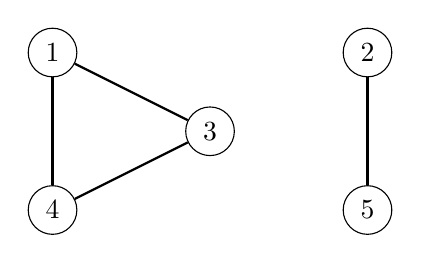
\begin{tikzpicture}
\node[draw, circle] (2) at (7,5) {$2$};
\node[draw, circle] (1) at (3,5) {$1$};
\node[draw, circle] (3) at (5,4) {$3$};
\node[draw, circle] (5) at (7,3) {$5$};
\node[draw, circle] (4) at (3,3) {$4$};

\path[draw,thick,-] (1) -- (3);
\path[draw,thick,-] (1) -- (4);
\path[draw,thick,-] (3) -- (4);
\path[draw,thick,-] (2) -- (5);
\end{tikzpicture}
\end{center}
es pot veure que una cerca en profunditat des del node $1$ visita els
nodes següents:
\begin{center}
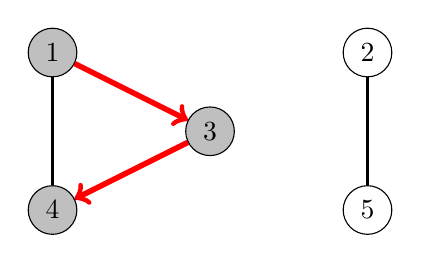
\begin{tikzpicture}
\node[draw, circle] (2) at (7,5) {$2$};
\node[draw, circle,fill=lightgray] (1) at (3,5) {$1$};
\node[draw, circle,fill=lightgray] (3) at (5,4) {$3$};
\node[draw, circle] (5) at (7,3) {$5$};
\node[draw, circle,fill=lightgray] (4) at (3,3) {$4$};

\path[draw,thick,-] (1) -- (3);
\path[draw,thick,-] (1) -- (4);
\path[draw,thick,-] (3) -- (4);
\path[draw,thick,-] (2) -- (5);

\path[draw=red,thick,->,line width=2pt] (1) -- (3);
\path[draw=red,thick,->,line width=2pt] (3) -- (4);

\end{tikzpicture}
\end{center}


Com que la cerca no ha visitat tots els nodes, en concloguem que el
graf no és connex. De manera semblant, podem trobar totes les
components connexes d'un graf iterant pels nodes i començant una nova
cerca en profunditat cada cop que trobem un node que no pertany a cap
component connexa.

\subsubsection{Trobar cicles}

\index{cicle}

Un graf conté un cicle si al recórrer el graf trobem un node amb un
veí que ja ha estat visitat, i que no sigui el node anterior en el
camí actual. Per exemple, el graf
\begin{center}
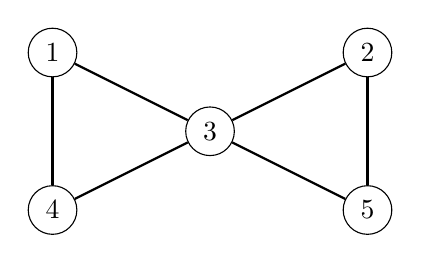
\begin{tikzpicture}
\node[draw, circle] (2) at (7,5) {$2$};
\node[draw, circle] (1) at (3,5) {$1$};
\node[draw, circle] (3) at (5,4) {$3$};
\node[draw, circle] (5) at (7,3) {$5$};
\node[draw, circle] (4) at (3,3) {$4$};

\path[draw,thick,-] (1) -- (3);
\path[draw,thick,-] (1) -- (4);
\path[draw,thick,-] (3) -- (4);
\path[draw,thick,-] (2) -- (5);
\path[draw,thick,-] (2) -- (3);
\path[draw,thick,-] (3) -- (5);
\end{tikzpicture}
\end{center}
conté dos cicles i podem trobar un d'ells de la següent manera:
\begin{center}
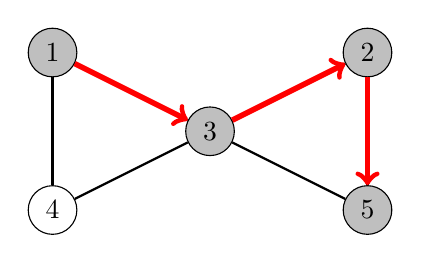
\begin{tikzpicture}
\node[draw, circle,fill=lightgray] (2) at (7,5) {$2$};
\node[draw, circle,fill=lightgray] (1) at (3,5) {$1$};
\node[draw, circle,fill=lightgray] (3) at (5,4) {$3$};
\node[draw, circle,fill=lightgray] (5) at (7,3) {$5$};
\node[draw, circle] (4) at (3,3) {$4$};

\path[draw,thick,-] (1) -- (3);
\path[draw,thick,-] (1) -- (4);
\path[draw,thick,-] (3) -- (4);
\path[draw,thick,-] (2) -- (5);
\path[draw,thick,-] (2) -- (3);
\path[draw,thick,-] (3) -- (5);

\path[draw=red,thick,->,line width=2pt] (1) -- (3);
\path[draw=red,thick,->,line width=2pt] (3) -- (2);
\path[draw=red,thick,->,line width=2pt] (2) -- (5);

\end{tikzpicture}
\end{center}
Després de passar del node 2 al node 5 observem que el veí 3 del node
5 ja ha estat visitat. Així, el graf conté un cicle que passa pel node
3, per exemple, $3 \rightarrow 2 \rightarrow 5 \rightarrow 3$.

Una altra manera d'esbrinar si un graf conté un cicle és calcular el
nombre de nodes i arestes de cada component connexa. Si un component
conté $c$ nodes i cap cicle, ha de contenir exactament $c-1$ arestes
(ha de ser un arbre). Si hi ha $c$ o més arestes, la component
sens dubte conté un cicle.

\subsubsection{Comprovar si un graf és bipartit}

\index{graf bipartit}

Un graf és bipartit si els seus nodes es poden acolorir amb dos colors
de manera que no hi hagi nodes adjacents amb el mateix
color. Comprovar si un graf és bipartit mitjançant algorismes de
recorregut de grafs és sorprenentment fàcil.

La idea és pintar el node inicial de blau, tots els seus veïns de
vermell, tots els seus veïns de blau, etc. Si en algun moment de la
cerca observem que dos nodes adjacents tenen el mateix color, això vol
dir que el graf no és bipartit. En cas contrari, el graf és bipartit i
hem trobat una coloració.

Per exemple, el graf
\begin{center}
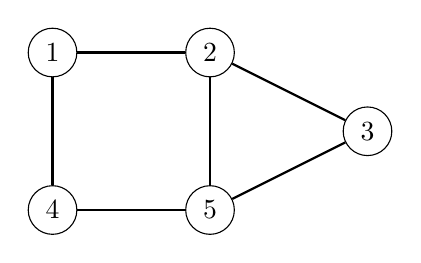
\begin{tikzpicture}
\node[draw, circle] (2) at (5,5) {$2$};
\node[draw, circle] (1) at (3,5) {$1$};
\node[draw, circle] (3) at (7,4) {$3$};
\node[draw, circle] (5) at (5,3) {$5$};
\node[draw, circle] (4) at (3,3) {$4$};

\path[draw,thick,-] (1) -- (2);
\path[draw,thick,-] (2) -- (5);
\path[draw,thick,-] (5) -- (4);
\path[draw,thick,-] (4) -- (1);
\path[draw,thick,-] (2) -- (3);
\path[draw,thick,-] (5) -- (3);
\end{tikzpicture}
\end{center}
no és bipartit, perquè si fem una cerca des del node 1 veiem el següent:
\begin{center}
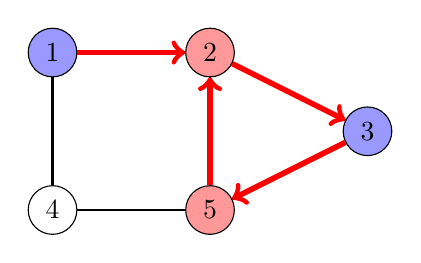
\begin{tikzpicture}
\node[draw, circle,fill=red!40] (2) at (5,5) {$2$};
\node[draw, circle,fill=blue!40] (1) at (3,5) {$1$};
\node[draw, circle,fill=blue!40] (3) at (7,4) {$3$};
\node[draw, circle,fill=red!40] (5) at (5,3) {$5$};
\node[draw, circle] (4) at (3,3) {$4$};

\path[draw,thick,-] (1) -- (2);
\path[draw,thick,-] (2) -- (5);
\path[draw,thick,-] (5) -- (4);
\path[draw,thick,-] (4) -- (1);
\path[draw,thick,-] (2) -- (3);
\path[draw,thick,-] (5) -- (3);

\path[draw=red,thick,->,line width=2pt] (1) -- (2);
\path[draw=red,thick,->,line width=2pt] (2) -- (3);
\path[draw=red,thick,->,line width=2pt] (3) -- (5);
\path[draw=red,thick,->,line width=2pt] (5) -- (2);
\end{tikzpicture}
\end{center}
Observem que el color dels nodes 2 i 5 és vermell, tot i que són
adjacents. Per tant, el graf no pot ser bipartit.

Aquest algorisme sempre funciona, perquè quan només hi ha dos colors
disponibles, el color del node inicial d'un component determina els
colors de tots els altres nodes del component, sense importat si
acolorim el node inicial vermell o blau.

Tingueu en compte que en el cas general, és difícil esbrinar si els
nodes d'un graf es poden acolorir amb $k$ colors de manera que cap
node adjacent tingui el mateix color. Fins i tot quan $k=3$, és sap
que el problema és NP-difícil i no es coneix cap algorisme eficient.


